\chapter{Số học}

\epigraph{{\rmfamily Toán học là vua của các môn khoa học, và số học là nữ hoàng}}{Carl Friedrich Gauss}

\begin{figure}[ht]
    \centering
    \fbox{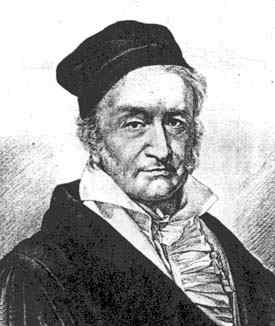
\includegraphics{mathematicians/Gauss.jpeg}}
    \captionsetup{labelformat=empty}
    \caption{Carl Friedrich Gauss (1777-1855)}
\end{figure}

\section{Phép chia Euclid và thuật toán Euclid}

\subsection*{Phép chia Euclid}

Đây là nền tảng, cơ sở của số học. Từ khi biết tới phép chia hai số nguyên, ta có thể tìm \textit{thương} và \textit{số dư}. Nói theo toán học, nếu ta có hai số nguyên dương $a$ và $b$ thì tồn tại cặp số $q$, $r$ sao cho $a = qb + r$ với $0 \leqslant r < b$.

Khi đó, $a$ gọi là số bị chia, $b$ gọi là số chia, $q$ là thương (q trong quotient) và $r$ là số dư (r trong remainder).

Đặc biệt là sự tồn tại của cặp số $q$ và $r$ là duy nhất. Thật vậy, nếu ta giả sử tồn tại 2 cặp số $(q_1, r_1)$ và $(q_2, r_2)$  đều thỏa đẳng thức trên, nghĩa là
\[a = q_1 b + r_1, \quad a = q_2 b + r_2\]

Trừ 2 đẳng thức vế theo vế ta có $(q_1 - q_2) b + (r_1 - r_2) = 0$. Tương đương $(r_2 - r_1) = (q_1 - q_2) b$, mà $0 \leqslant r_1, r_2 < b$ nên $-b < r_2 - r_1 < b$. Như vậy chỉ có thể xảy ra trường hợp
$r_2 - r_1 = 0$ hay $r_2 = r_1$, kéo theo $q_1 = q_2$.

\subsection*{Thuật toán Euclid}

Dựa trên phép chia Euclid, ta có một thuật toán hiệu quả để tìm ước chung lớn nhất giữa hai số $a$ và $b$.

Ký hiệu $\gcd(a, b)$ là ước chung lớn nhất của $a$ và $b$. Chúng  ta thực hiện đệ quy như sau:
\begin{equation*}
    \gcd(a, b) = \begin{cases}
        a, \quad & \text{nếu}\,b = 0 \\
        \gcd(b, a \bmod b), \quad & \text{nếu}\,b \neq 0
    \end{cases} 
\end{equation*}

Điểm quan trọng ở thuật toán Euclid là thuật toán chắc chắn sẽ dừng sau một số hữu hạn bước, và kết quả sẽ là ước chung lớn nhất của hai số $a$ và $b$.

\begin{proof}
    Đặt $r_0 = a$ và $r_1 = b$. Theo thuật chia Euclid ta có các số $q_0$ và $r_2$ sao cho $r_0 = r_1 q_0 + r_2$ với $0 \leqslant r_2 < r_1$. Thuật toán Euclid hoạt động như sau:
    \begin{align*}
        r_0 & = r_1 q_0 + r_2 \\
        r_1 & = r_2 q_1 + r_3 \\
        r_2 & = r_3 q_2 + r_4 \\
        \ldots & = \ldots \\
        r_i & = r_{i+1} q_i + r_{i+2} \\
        \ldots & = \ldots \\
        r_k & = r_{k+1} q_k + 0 \\
        r_{k+1} & = 0
    \end{align*}
    Ta thấy rằng ở mỗi bước, $r_{i+2}$ luôn nhỏ hơn $r_{i+1}$. Do đó cuối cùng sẽ bằng 0, và khi đó ta có ước chung lớn nhất.
\end{proof}

\subsection*{Thuật toán Euclid mở rộng}

\begin{definition}[Phương trình Diophantos]
    Cho trước các số nguyên $a$, $b$ và $c$. Phương trình  Diophantus là phương trình có dạng
    \[ax + by = c\]
    với $x$, $y$ là các số nguyên.
\end{definition}

\begin{example}
    Giải phương trình $5x+3y = 1$.

    Ta có $y = \dfrac{1-5x}{3} = \dfrac{1-2x-3x}{3} = \dfrac{1-2x}{3} - x$. Như vậy nếu $y \in \ZZ$ thì $\dfrac{1-2x}{3} \in \ZZ$, nghĩa là $1-2x$ chia hết cho 3. Vậy $1-2x = 3k$ với $k \in \ZZ$.

    Tiếp tục, $1-2x = 3k$, suy ra $x = \dfrac{1-3k}{2}  = \dfrac{1-k-2k}{2} = \dfrac{1-k}{2} - k$. Do $x$ nguyên nên tương tự $\dfrac{1-k}{2}$ cũng nguyên, hay $1-k = 2t$, tương đương với $k = 1-2t$.

    Thay ngược lại ta có $x = \dfrac{1-3k}{2} = \dfrac{1-3(1-2t)}{2} = {-1+3t}$. Tiếp tục thay vào để tìm $y$ thì $y = \dfrac{1-5x}{3} = \dfrac{1-5(-1+3t)}{3} = 2 - 5t$.

    Như vậy nghiệm của phương trình là tất cả các nghiệm $(x, y)$ mà $x = -1+3t$, $y = 2-5t$ với $t \in \ZZ$.
\end{example}

Ở đây chúng ta đã thực hiện phép chia có dư liên tiếp để tìm nghiệm. Nói cách khác ta đã thực hiện thuật toán Euclid ở bên trên để làm giảm độ phức tạp ở mỗi bước giải. Tổng quát ta có thuật toán Euclid mở rộng để tìm ước chung lớn nhất $\gcd(a, b)$ của hai số $a$, $b$, và \textbf{một} nghiệm của phương trình $ax + by = \gcd(a, b)$.

Ở ví dụ trên, ta thấy rằng $(-1, 2)$ là một nghiệm của phương trình $5x + 3y = 1$. Khi đó ta có thể suy ra tất cả nghiệm (họ nghiệm) của phương trình có dạng $(-1+3t, 2-5t)$ với $t \in \ZZ$.

\begin{algorithm}
    \caption{Thuật toán Euclid mở rộng}
    \begin{algorithmic}
        \Require $a, b \in \ZZ$
        \Ensure $\gcd(a, b)$, $x$, $y$ 
        \State $r_0 \gets a$, $r_1 \gets b$, $r_2 \gets 0$
        \State $x_0 \gets 1$, $x_1 \gets 0$, $x_2 \gets 0$
        \State $y_0 \gets 0$, $y_1 \gets 1$, $y_2 \gets 0$
        \While{$r_1 \neq 0$}
            \State $q \gets r_0 \;\text{div}\; r_1$
            \State $r_2 \gets r_0 - q * r_1$, $r_0 \gets r_1$, $r_1 \gets r_2$
            \State $x_2 \gets x_0 - q * x_1$, $x_0 \gets x_1$, $x_1 \gets x_2$
            \State $y_2 \gets y_0 - q * y_1$, $y_0 \gets y_1$, $y_1 \gets y_2$
        \EndWhile
        \State \Return $r_0$, $x_0$, $y_0$
    \end{algorithmic}
\end{algorithm}

Ở thuật toán trên, $r_0$, $r_1$ và $r_2$ hoạt động như thuật toán Euclid chuẩn. Ở mỗi bước $q$ là thương của phép chia hai số nguyên và ta sử dụng $q$ đó để tính $x_0$ và $y_0$ mới. Kết quả cuối cùng $(r_0, x_0, y_0)$ lần lượt là ước chung lớn nhất, và hai số $x$, $y$ thỏa mãn $a x_0 + y b_0 = r_0$.

Tại sao chúng ta lại có $(x_0, x_1) = (1, 0)$ và $(y_0, y_1) = (0, 1)$? Nói cách khác, làm sao biết thuật toán  hoạt động đúng?

Mục đích của chúng ta là tìm các số $(x, y)$ sao cho $ax + by = \gcd(a, b)$. Khi đó, dựa trên thuật toán Euclid cơ bản ở trên, ta xây dựng dãy số $\{x_n\}$ và $\{y_n\}$ sao cho ở mọi bước thứ $n$ ta đều có

\begin{equation}\label{euclid:1}
    a x_n + b y_n = r_n
\end{equation}

Ta có $r_i = r_{i+1} q_i + r_{i+2}$. Từ $q_i$ ở mỗi bước ta tính được
\begin{equation*}
    x_i = x_{i+1} q_i + x_{i+2}, \quad y_i = y_{i+1} q_i + y_{i+2}
\end{equation*}

Thay vào \ref{euclid:1} ta được
\begin{equation}
    a (x_{i+1} q_i + x_{i+2}) + b (y_{i+1} q_i + y_{i+2}) = r_i
\end{equation}

Tương đương với \[(a x_{i+1} + b y_{i+1}) q_i + (a x_{i+2} + b x_{i+2}) = r_i\]

Mà $a x_{i+1} + b y_{i+1} = r_{i+1}$ và $a x_{i+2} + b y_{i+2} = r_{i+2}$. Suy ra $r_{i+1} q_i + r_{i+2} = r_n$, đúng với thuật toán Euclid chuẩn ban đầu. Nghĩa là thuật toán hoạt động đúng. Bây giờ ta cần chọn $(x_0, x_1)$ và $(y_0, y_1)$ vì chúng ta đã đặt $r_0 = a$ và $r_1 = b$. Ở bước thứ 0, \[r_0 = a = a x_0 + b y_0\] và ở bước thứ 1,
\[r_1 = b = a x_1 + b y_1\]

Dễ thấy ở bước 0 ta chọn $(1, 0)$ và ở bước 1 ta chọn $(0, 1)$ là được.

\section{Hàm Euler}

\begin{definition}[Phi hàm Euler]
    Cho số nguyên dương $n$. Số lượng các số dương nhỏ hơn $n$ và nguyên tố cùng nhau với $n$ được ký hiệu bởi $\varphi(n)$ và gọi là $\varphi$ hàm Euler. \[ \varphi(n) = \lvert \{ a : (a, n) = 1\} \rvert \]
\end{definition}   

Hàm Euler có ý nghĩa quan trọng trong lý thuyết số, công cụ giúp chúng ta giải các vấn đề về số mũ trong modulo.

Sau đây chúng ta xem xét hệ thặng dư đầy đủ và hệ thặng dư thu gọn.

Với số nguyên dương $n$, ta định nghĩa

\begin{definition}[Hệ thặng dư đầy đủ]
    Hệ thặng dư đầy đủ của $n$ là tập $\{0, 1, \ldots, n-1\}$.
\end{definition}

Nói cách khác, hệ thặng dư đầy đủ của $n$ là các số dư có thể có khi chia một số bất kì cho $n$.

\begin{definition}[Hệ thặng dư thu gọn]
    Hệ thặng dư thu gọn của $n$ là tập các số $a$ mà $1 \leqslant a < n$ và $(a, n) = 1$. Số lượng các số $a$ như vậy là $\varphi (n)$.  
\end{definition}

\begin{remark}
    \begin{enumerate}
        \item Hệ thặng dư thu gọn của $n$ gồm $\varphi(n)$ phần tử là \[ \{a_1, a_2, \ldots, a_{\varphi(n)}\} \]
        \item Nếu $n$ là số nguyên tố thì $\varphi(n) = n-1$.
    \end{enumerate}
\end{remark}

\subsection*{Tính chất hàm Euler}

\begin{remark}
    Với $(m, n) = 1$ thì $\varphi(m n) = \varphi(m) \varphi(n)$.
\end{remark}

\begin{proof}
    Ta viết các số từ 1 tới $mn$ thành bảng như sau

    \begin{table}
        \centering
        \begin{tabular}{c c c c}
            1 & $m+1$ & $\cdots$ & $(n-1)m + 1$ \\
            2 & $m+2$ & $\cdots$ & $(n-1)m + 2$ \\
            $\cdots$ & $\cdots$ & $\cdots$ & $\cdots$ \\
            $m$ & $m+m$ & $\cdots$ & $(n-1)m + m$
        \end{tabular}
    \end{table}
    
    Hàng $r$ gồm các phần tử dạng $r m + k$ với $0 \leqslant r \leqslant n-1$ và $1 \leqslant k \leqslant m$.  Ta thấy rằng nếu $(rm + k, m) = 1$ thì $(k, m) = 1$.

    Do đó trên mỗi hàng có $\varphi(m)$ phần tử nguyên tố cùng nhau với $m$.

    Tiếp theo, trên các hàng vừa tìm được, do $(m, n) = 1$ nên để $(rm + k, n) = 1$ thì $(r, n) = 1$. Nghĩa là có $\varphi(n)$ hàng như vậy.

    Tổng kết lại, ta có $\varphi(m) \varphi(n)$ phần tử trong bảng nguyên tố cùng nhau với $mn$. Do đó có điều phải chứng minh.
\end{proof}

Do tính chất này nên hàm Euler là hàm nhân tính.

\begin{remark}
    Cho số nguyên dương $n$. Khi đó $\displaystyle{\sum_{d | n} \varphi(d) = n}$.
\end{remark}

\begin{proof}
    Giả sử phân tích thừa số nguyên tố của $n$ là 
    \begin{equation*}
        n = p_1^{e_1} p_2^{e_2} \ldots p_k^{e_k}
    \end{equation*}

    Khi đó mỗi ước $d$ của $n$ đều có dạng $p_1^{f_1} p_2^{f_2} \ldots p_k^{f_k}$ với $0 \leqslant f_i \leqslant e_i$ với $i = 1, 2, \ldots, k$.

    Như vậy
    \begin{equation*}
        \sum_{d | n} \varphi(d) = \sum_{0 \leqslant f_i \leqslant e_i} \varphi\Big(p_1^{f_1} p_2^{f_2} \ldots p_k^{f_k}\Big)
                            = \varphi\Big(p_1^{f_1}\Big) \varphi\Big(p_2^{f_2}\Big) \ldots \varphi\Big(p_k^{f_k}\Big)
    \end{equation*}

    Một dạng biểu thức đơn giản là $(1+x)(1+y) = 1+x+y+xy$ hay với 3 biến là $(1+x)(1+y)(1+y) = 1 + x + y + z + xy + yz + yz + xyz$. Tổng quát cho $k$ biến ở trên thì biểu thức tương đương với
    \begin{align*}
        \sum_{0 \leqslant f_i \leqslant e_i} \varphi(p_1^{f_1}) \varphi(p_2^{f_2}) \ldots
        \varphi(p_k^{f_k}) = & (1 + \varphi(p_1) + \varphi(p_1^2) + \ldots + \varphi(p_1^{e_1})) \\
        \times & (1 + \varphi(p_2) + \varphi(p_2^2) + \ldots + \varphi(p_2^{e_2})) \\
        \times & \ldots \\
        \times & (1 + \varphi(p_k) + \varphi(p_k^2) + \ldots + \varphi(p_k^{e_k}))
    \end{align*}

    Ở đây ta rút gọn dễ dàng với $i = 1, 2, \ldots, k$:
    \begin{align*}
        & 1 + \varphi(p_i) + \varphi(p_i^2) + \ldots + \varphi(p_i^{e_i}) \\
        = & 1 + p_i - 1 + p_i^2 - p_i + \ldots + p_i^{e_i} - p_i^{e_i-1} \\
        = & p_i^{e_i}
    \end{align*}

    Như vậy mỗi tổng $1 + \varphi(p_i) + \ldots$ bằng chính $p_i^{e_i}$. Nhân chúng lại với nhau ta có lại $n$.
\end{proof}

\subsection*{Định lý Euler}

\begin{theorem}[Định lý Euler]    
    Cho số nguyên dương $n$. Với mọi số nguyên $a$ mà $(a, n) = 1$ thì 
    \begin{equation}
        a^{\varphi(n)} \equiv 1 \pmod n
    \end{equation}
\end{theorem}

\begin{proof}
    Giả sử $S = \{a_1, a_2, \ldots, a_{\varphi(n)}\}$ là hệ thặng dư thu gọn của $n$. Ta sẽ chứng minh rằng nếu $a$ là số sao cho $(a, n)=1$ thì tập hợp
    \begin{equation*}
        \{a a_1, a a_2, \ldots, a a_{\varphi(n)}\}
    \end{equation*}
    là hoán vị của tập $S$.

    Thật vậy, giả sử $a a_i \equiv a a_j \pmod n$ với $1 \leqslant i, j \leqslant \varphi(n)$ và $i \neq j$.

    Do $(a, n) = 1$ nên tồn tại nghịch đảo $a' \pmod n$, nhân $a'$ cho 2 vế ta còn $a_i \equiv a_j \pmod n$.

    Nói cách khác, nếu $a_i \not\equiv a_j \pmod n$ thì $a a_i \not\equiv a a_j \pmod n$. Suy ra tập
    \begin{equation*}
        \{a a_1, a a_2, \ldots, a a_{\varphi(n)}\}
    \end{equation*}
    là hoán vị của $S$.

    Ta nhân tất cả phần tử của $S$ thì sẽ bằng tích phần tử của tập trên
    \begin{equation*}
        a a_1 \cdot a a_2 \ldots a a_{\varphi(n)} \equiv a_1 \cdot a_2 \ldots a_{\varphi(n)} \pmod n
    \end{equation*}

    Đặt $I = a_1 \cdot a_2 \ldots a_{\varphi(n)}$ thì phương trình trên tương đương với 
    \begin{equation*}
        a^{\varphi(n)} I \equiv I \pmod n
    \end{equation*}
    
    Mà $(I, n) = 1$ do là tích các số nguyên tố cùng nhau với $n$ nên rút gọn hai vế ta được
    \begin{equation*}
        a^{\varphi(n)} \equiv 1 \pmod n
    \end{equation*}
    Ta có điều phải chứng minh.
\end{proof}

\subsection*{Định lý Fermat nhỏ}

\begin{theorem}[Định lý Fermat nhỏ]    
    Cho số nguyên tố $p$. Với mọi số nguyên $a$ thì $$a^p \equiv a \pmod p$$

    Khi $(a, p) = 1$ thì
    \begin{equation*}
        a^{p-1} \equiv 1 \pmod p
    \end{equation*}
\end{theorem}

\begin{remark}
    Khi $(a, p) = 1$ thì định lý Fermat là hệ quả trực tiếp từ định lý Euler.
\end{remark}

\section{Thặng dư chính phương}

\begin{definition}[Số chính phương modulo $p$]
    Xét số dương nguyên tố lẻ $p$. Số $a$ được gọi là \textbf{số chính phương modulo $p$} nếu $(a, m) = 1$ và tồn tại số $x$ sao cho $x^2 = a \pmod p$.

    Nói cách khác phương trình đồng dư $x^2 \equiv a \pmod p$ có nghiệm.
\end{definition}

Chúng ta sử dụng kí hiệu Legendre (Legendre symbol) để thể hiện một số $a$ có phải là số chính phương modulo nguyên tố $p$ không.

\begin{definition}[Legendre symbol]
    Xét $p$ là số nguyên tố, $a$ là số nguyên không chia hết cho $p$. Khi đó kí hiệu Legendre được định nghĩa là
    \begin{equation}
        \left(\frac{a}{p}\right) = \begin{cases}
            1, & \text{ nếu } a \text{ là số chính phương modulo } p. \\
            -1, & \text{ nếu ngược lại.}
        \end{cases}
    \end{equation}
\end{definition}

Một trường hợp tổng quát hơn của kí hiệu Legendre là kí hiệu Jacobi áp dụng cho số nguyên dương bất kì.
\begin{definition}[Jacobi symbol]
    Xét $n$ là số nguyên dương, $a$ là số nguyên không chia hết cho $n$. Khi đó kí hiệu Jacobi được định nghĩa là
    \begin{equation}
        \left(\frac{a}{n}\right) = \begin{cases}
            1, & \text{ nếu } a \text{ là số chính phương modulo } n \\
            -1, & \text{ nếu ngược lại.}
        \end{cases}
    \end{equation}
\end{definition}

\section{Hàm Möbius}

August Ferdinand Möbius là nhà toán học người Đức, đóng góp nổi tiếng của ông là dải Möbius. Tuy nhiên ở đây chúng ta xem xét một hàm số học mang tên ông. 

Hàm Möbius đóng vai trò quan trọng trong việc tính các đại lượng liên quan tới số học.

\subsection*{Hàm Möbius}

\begin{definition}[Hàm Möbius]
    Hàm Möbius của số nguyên dương $n$ được định nghĩa như sau:
    \begin{equation}
        \mu (n) = \begin{cases}
            1, \quad & \text{nếu}\, n = 1 \\
            (-1)^k, \quad & \text{nếu}\, n = p_1 p_2 \ldots p_k  \text{ với } p_i \text{ là số nguyên tố} \\
            0, \quad & \text{trong các trường hợp còn lại}
        \end{cases}
    \end{equation}
\end{definition}

Điều này có nghĩa là, nếu $n$ là tích của các số nguyên tố bậc 1 thì $\mu (n) = (-1)^k$ với $k$ là số lượng số nguyên tố trong tích. Như vậy, nếu tồn tại số nguyên tố $p$ sao cho $p^2 \mid n$ thì $\mu(n) = 0$.

\subsection*{Tính chất hàm Möbius}

\begin{enumerate}
    \item Nếu $(n_1, n_2) = 1$ thì $\mu(n_1, n_2) = \mu(n_1) \mu(n_2)$
    \item $\displaystyle{\sum_{d \mid n} \mu(d) = 0}$ với $n = p_1 p_2 \ldots p_k$
\end{enumerate}

\begin{proof}
    Với tính chất 1, ta dễ thấy rằng do $n_1$ và $n_2$ nguyên tố cùng nhau nên trong
    cách phân tích thừa số nguyên tố của chúng sẽ chứa các số nguyên tố khác nhau. 
    Khi đó $\mu(n_1)$ và $\mu(n_2)$ không bị phụ thuộc nhau và có thể tách thành phép
    nhân như trên.

    Với tính chất 2, chúng ta lần lượt chọn $d$ là tổ hợp của 0, 1, 2, ..., $k$
    số nguyên tố.

    \begin{itemize}
        \item Nếu $d = 1$ thì $\mu(d) = 1$
        \item Nếu $d = p_i$ thì $\mu(d) = (-1)^1 = -1$ với $i = \overline{1, k}$
        \item Nếu $d = p_i p_j$ với $i \neq j$ thì $\mu (d) = (-1)^2 = 1$
        \item Tương tự như vậy, nếu $d$ là tích của $t$ số nguyên tố thì
        $\mu (d) = (-1)^t$
    \end{itemize}

    Ở mỗi trường hợp trên, do $d$ là tổ hợp của $t$ số nguyên tố ($0 \leqslant t \leqslant k$)
    nên số cách chọn số nguyên tố $p_i$ ở mỗi trường hợp là $C^t_k$. Cộng chúng lại

    \[\sum_{d \mid n} \mu(d) = 1 - C^1_k + C^2_k - \ldots + (-1)^k C^k_k = 0\]
    theo nhị thức Newton. Từ đó ta có điều phải chứng minh.
\end{proof}

\subsection*{Công thức nghịch đảo Möbius}

Giả sử ta có hai hàm $f$ và $g$ từ $\NN \to \ZZ$. Khi đó hai cách biểu diễn sau
là tương đương.
\begin{equation}
    f(n) = \sum_{d \mid n} g(d) \Leftrightarrow g(n) 
    = \sum_{d \mid n} f(d) \mu\left(\frac{n}{d}\right)
\end{equation}

Nghĩa là nếu chúng ta có hai hàm số $f$ và $g$ thỏa phương trình đầu (biểu diễn
$f$ theo $g$) thì chúng ta cũng sẽ tìm được cách biểu diễn $g$ theo $f$.

\begin{proof}
    Với $d \mid n$, đặt $d' = \dfrac{n}{d} \Rightarrow d = \dfrac{n}{d'}$.

    Suy ra $f(d) \cdot \mu\left(\dfrac{n}{d}\right) = 
    f \left(\dfrac{n}{d'}\right) \cdot \mu(d')$.
    Sau đó lấy tổng lại thì

    \[\sum_{d \mid n} f(d) \cdot \mu \left(\frac{n}{d}\right) = 
    \sum_{d \mid n} f\left(\frac{n}{d'}\right) \cdot  \mu(d') = 
    \sum_{d \mid n} f\left(\frac{n}{d}\right) \cdot \mu(d)\]
    
    Ở đây lưu ý rằng nếu $d$ là ước của $n$ thì $d' = \dfrac{n}{d}$ cũng là
    ước của $n$. Do đó ta hoàn toàn có thể thay thế $d'$ bởi $d$ trong tổng trên.

    Vì $f(n) = \displaystyle{\sum_{d \mid n} g(d)}$ nên 
    \begin{equation}
        \label{eq:mebius1}
        \sum_{d \mid n} f\left(\frac{n}{d}\right) \cdot \mu(d)
    = \sum_{d \mid n} \mu(d) \sum_{d' \mid \frac{n}{d}} g(d')
    \end{equation}

    Dễ thấy rằng do $d \mid n$ và $d' \mid \dfrac{n}{d}$ nên tồn tại
    $k$, $l$ sao cho $kd = n$ và $ld' = \dfrac{n}{d}$. Khi đó $n = ldd'$ và $kd = n$.
    Suy ra $d' \mid n$ và $d \mid \dfrac{n}{d'}$.

    Tương tự như trên, ta có thể thay thế $d$ bởi $d'$ và ngược lại
    \[(\ref{eq:mebius1}) = \sum_{d' \mid n} g(d') \sum_{d \mid \frac{n}{d'}} \mu(d)\]
    mà $\displaystyle{\sum_{a \mid p} \mu(a) = 0}$ nếu $p \neq 1$ và bằng 1 với $p = 1$.
    (đã chứng minh ở trên), nên từ đây suy ra
    \[
        \sum_{d' \mid n} g(d') \sum_{d \mid \frac{n}{d'}} \mu(d)
        = \sum_{d' \mid n} g(d') \cdot 1 \,(\text{khi } n = d') = g(n)    
    \]
\end{proof}

Tương tự ta cũng có công thức nghịch đảo Möbius đối với phép nhân
\begin{equation}
    f(n) = \prod_{d \mid n} g(d) \Leftrightarrow 
    g(n) = \prod_{d \mid n} f(d)^{\mu\left(\frac{n}{d}\right)}
\end{equation}

\textbf{Liên hệ với hàm Euler}

Nếu ta chọn $f(n) = n$ và $g(n) = \varphi(n)$ thì theo công thức nghịch đảo Möbius ta có
$\displaystyle{\varphi(n) = \sum_{d \mid n} d \cdot \mu\left(\frac{n}{d}\right)}$
do ta đã biết $\displaystyle{\sum_{d \mid n} \varphi(d) = n}$.

\section{Định lý số dư Trung Hoa}

Định lý số dư Trung Hoa (Chinese Remainder Theorem - CRT) là một trong những định lý quan trọng nhất của số học nói riêng và toán học nói chung.

\subsection*{Chứng minh định lý số dư Trung Hoa}

Giả sử ta có hệ phương trình đồng dư
\begin{align*}
	x & \equiv x_1 \pmod{m_1} \\ x & \equiv x_2 \pmod{m_2} \\ & \ldots \\ x & \equiv x_k \pmod{m_k}
\end{align*}

Trong đó $\gcd(m_i, m_j) = 1$ với mọi $i \neq j$, $1 \leqslant i, j \leqslant k$.

Khi đó định lý số dư Trung Hoa phát biểu rằng hệ phương trình đồng như này có nghiệm duy nhất trong modulo $M = m_1 m_2 \ldots m_k$.

\begin{proof}
	Chúng ta cần chứng minh sự tồn tại và tính duy nhất của nghiệm.
	
	Để chứng minh sự tồn tại, ta xây dựng cách tính nghiệm bằng quy nạp.
	
	\underline{Bước cơ sở}. Với $k=2$, ta có $x \equiv x_1 \pmod{m_1}$ và $x \equiv x_2 \pmod{m_2}$. Do $\gcd(m_1, m_2) = 1$ nên tồn tại hai số nguyên $n_1$, $n_2$ sao cho $m_1 n_1 + m_2 n_2 = 1$ (bổ đề Bézout).
	
	Quan sát một chút, nếu ta modulo hai vế $m_1 n_1 + m_2 n_2 = 1$ cho $m_1$ thì sẽ có $m_2 n_2 \equiv 1 \pmod{m_1}$. Như vậy $x \equiv x_1 \cdot 1 \pmod{m_1} \Leftrightarrow x \equiv x_1 \cdot (m_2 n_2) \pmod{m_1}$ (?).
	
	Tương tự, $m_1 n_1 \equiv 1 \pmod{m_2}$ nên $x \equiv x_2 \cdot 1 \pmod{m_2} \Leftrightarrow x \equiv x_2 \cdot (m_1 n_1) \pmod{m_2}$.
	
	Từ đó ta có công thức nghiệm là \[x \equiv x_1 m_2 n_2 + x_2 m_1 n_1 \pmod{m_1 m_2}\]
	Khi modulo cho $m_1$ và $m_2$ thì kết quả là hai phương trình đồng dư ban đầu.
	
	Tiếp theo chúng ta sử dụng quy nạp để chứng minh với mọi $k \geqslant 2$ thì nghiệm của hệ phương trình đồng dư là
	\begin{equation}
		\label{crt:eq1}
		x \equiv x_1 M_1 N_1 + x_2 M_2 N_2 + \ldots + x_k M_k N_k \pmod{M}
	\end{equation}
	
	Trong đó $M = m_1 \cdot m_2 \cdots m_k$, $M_i = M / m_i$, $N_i$ là nghịch đảo của $M_i$ trong modulo $m_i$
	
	\underline{Giả thiết quy nạp}. Giả sử \ref{crt:eq1} đúng với $k \geqslant 2$. Đặt $M = m_1 \cdots m_k$ và $X_k = x_1 M_1 N_1 + \ldots +  x_k M_k N_k$. Với $k+1$ ta có
	\begin{align*}
		x & \equiv X_k \pmod{M} \\ x & \equiv x_{k+1} \pmod{m_{k+1}}
	\end{align*}
	
	Tương tự với hai modulo ở trên, do $\gcd(m_{k+1}, m_i) = 1$ với mọi $1 \leqslant i \leqslant k$ nên $\gcd(m_{k+1}, m_1 \cdots m_k) = \gcd(m_{k+1}, M) = 1$. Khi đó tồn tại các số nguyên $\alpha$ và $\beta$ sao cho $\alpha M + \beta m_{k+1} = 1$.
	
	Nghiệm của hệ hai phương trình đồng dư khi này là
	\begin{equation*}
		x \equiv X_k \beta m_{k+1} + x_{k+1} \alpha M \pmod{M \cdot m_{k+1}}
	\end{equation*}
	
	Đặt $M' = M \cdot m_{k+1} = m_1 \cdots m_k \cdot m_{k+1}$. Ở đây $M = M' / m_{k+1}$ chính là $M'_{k+1}$ trong cách xây dựng nghiệm ở trên. Từ đó $\alpha$ chính là $N'_{k+1}$.
	
	Ta có $X_k \beta m_{k+1} = (x_1 M_1 N_1 + \ldots + x_k M_k N_k) \beta m_{k+1}$. Để ý rằng $M_i = M / m_i = M' / (m_i \cdot m_{k+1})$ nên $M_i \cdot m_{k+1} = M' / m_i = M'_i$. 
	
	Tiếp theo, do $\beta m_{k+1} \equiv 1 \pmod{M}$ và $M = m_1 \cdots m_k$ nên $\beta m_{k+1} \equiv 1 \pmod{m_i}$ với $1 \leqslant i \leqslant k$. Ở trên ta có $N_i M_i \equiv 1 \pmod{m_i}$ nên suy ra $\beta m_{k+1} \cdot N_i M_i \equiv 1 \pmod{m_i}$. Tương đương với $(\beta N_i) \cdot (M_i m_{k+1}) \equiv 1 \pmod{m_i}$. Ta đã chứng minh ở trước $M_i m_{k+1} = M'/m_i = M'_i$ nên $\beta N_i = N'_i$. Tới đây thì ta đã hoàn thành chứng minh do
	\begin{align*}
		& X_k \cdot \beta \cdot m_{k+1} + x_{k+1} \cdot \alpha \cdot M \\ 
        = & (x_1 M_1 N_1 + \ldots + x_k M_k N_k) \cdot \beta \cdot m_{k+1} + x_{k+1} \cdot N'_{k+1} \cdot M'_{k+1} \\ 
        = & x_1 \cdot (\beta N_1) \cdot (M_1 m_{k+1}) + \ldots + x_k \cdot (\beta N_k) \cdot (M_k m_{k+1}) \\ 
        & + x_{k+1} \cdot N'_{k+1} \cdot M'_{k+1} \\ 
        = & x_1 N'_1 M'_1 + \ldots x_k N'_k M'_k + x_{k+1} N'_{k+1} M'_{k+1}
	\end{align*}
	
	Để chứng minh sự duy nhất của nghiệm, giả sử $y$ là một nghiệm khác $x$ của hệ phương trình đồng dư (modulu $M$). Khi đó $y \equiv x_i \equiv x \pmod{m_i}$. Như vậy $y = x + t_i m_i$, hay nói cách khác $y$ khác $x$ một bội của $m_i$. Do đó trong modulo $m_i$ chỉ có thể có trường hợp $y \equiv x$ nên nghiệm tìm được ở modulo tổng là duy nhất.
\end{proof}

\begin{example}
	Tìm nghiệm của hệ phương trình đồng dư sau
	\begin{align*}
		x \equiv 1 \pmod 3 \\
		x \equiv 4 \pmod 7
	\end{align*}
	
	Ta có $\gcd(3, 7) = 1$ và $3 \cdot 5 + 7 \cdot (-2) = 1$. Do đó nghiệm của hệ phương trình có dạng 
	\[x \equiv 1 \cdot 7 \cdot (-2) + 4 \cdot 3 \cdot 5 = 4 \pmod{21}\]
	
	Ta thấy rằng $4 \equiv 1 \pmod 3$ và $4 \equiv 4 \pmod 7$ thỏa mãn hệ phương trình đồng dư.
\end{example}